\documentclass[tikz,border=2pt]{standalone}
\usepackage{tikz}
\usepackage{helvet}
\renewcommand{\familydefault}{\sfdefault}

\definecolor{geo}{HTML}{0072B2}
\definecolor{evq}{HTML}{E69F00}
\definecolor{delta}{HTML}{009E73}
\definecolor{grid}{HTML}{D9D9D9}

\begin{document}
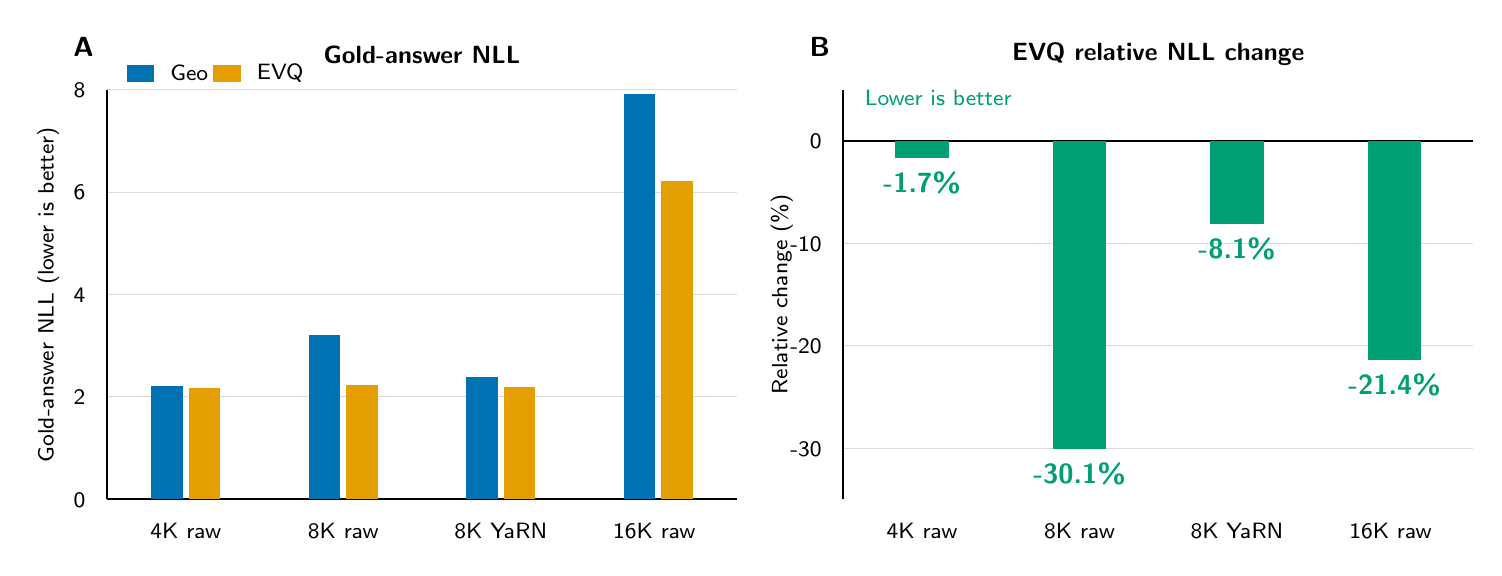
\begin{tikzpicture}[font=\sffamily\fontsize{8}{9}\selectfont]
  % Panel A: table values, Gold-answer NLL.
  \begin{scope}
    \node[font=\bfseries\fontsize{10}{11}\selectfont,anchor=west] at (-0.55,5.75) {A};
    \node[font=\bfseries\fontsize{9}{10}\selectfont] at (4.0,5.65) {Gold-answer NLL};
    \foreach \v in {0,2,4,6,8} {
      \draw[grid,line width=0.35pt] (0,{0.65*\v}) -- (8,{0.65*\v});
      \node[anchor=e] at (-0.15,{0.65*\v}) {\v};
    }
    \draw[line width=0.7pt] (0,0) -- (8,0);
    \draw[line width=0.7pt] (0,0) -- (0,5.2);
    \node[rotate=90] at (-0.75,2.6) {Gold-answer NLL (lower is better)};

    \foreach \x/\g/\e/\lab in {
      1/1.443/1.418/{4K raw},
      3/2.081/1.455/{8K raw},
      5/1.553/1.427/{8K YaRN},
      7/5.145/4.043/{16K raw}
    } {
      \fill[geo] (\x-0.44,0) rectangle (\x-0.04,\g);
      \fill[evq] (\x+0.04,0) rectangle (\x+0.44,\e);
      \node[align=center,anchor=north] at (\x,-0.18) {\lab};
    }
    \fill[geo] (0.25,5.30) rectangle (0.60,5.52);
    \node[anchor=west] at (0.68,5.41) {Geo};
    \fill[evq] (1.35,5.30) rectangle (1.70,5.52);
    \node[anchor=west] at (1.78,5.41) {EVQ};
  \end{scope}

  % Panel B: relative NLL change from the same four Table 21 rows.
  \begin{scope}[xshift=9.35cm]
    \node[font=\bfseries\fontsize{10}{11}\selectfont,anchor=west] at (-0.55,5.75) {B};
    \node[font=\bfseries\fontsize{9}{10}\selectfont] at (4.0,5.65) {EVQ relative NLL change};
    \foreach \v in {-30,-20,-10,0} {
      \draw[grid,line width=0.35pt] (0,{4.55+0.13*\v}) -- (8,{4.55+0.13*\v});
      \node[anchor=e] at (-0.15,{4.55+0.13*\v}) {\v};
    }
    \draw[line width=0.7pt] (0,0) -- (0,5.2);
    \draw[line width=0.7pt] (0,4.55) -- (8,4.55);
    \node[rotate=90] at (-0.78,2.6) {Relative change (\%)};
    \node[anchor=west,text=delta] at (0.15,5.10) {Lower is better};

    \foreach \x/\bottom/\value/\lab in {
      1/4.329/{-1.7\%}/{4K raw},
      3/0.637/{-30.1\%}/{8K raw},
      5/3.497/{-8.1\%}/{8K YaRN},
      7/1.768/{-21.4\%}/{16K raw}
    } {
      \fill[delta] (\x-0.34,\bottom) rectangle (\x+0.34,4.55);
      \node[font=\bfseries,anchor=north,text=delta] at (\x,\bottom-0.05) {\value};
      \node[align=center,anchor=north] at (\x,-0.18) {\lab};
    }
  \end{scope}
\end{tikzpicture}
\end{document}
